\documentclass[11pt]{article}
\usepackage[a4paper,margin=1in]{geometry}
\usepackage{amsmath,amssymb,bm}
\usepackage{graphicx}
\usepackage{booktabs}
\usepackage{hyperref}
\usepackage{array}

\title{HHL Algorithm in Qiskit:\\From Quantum Linear Systems to Executable Circuits}
\author{Compact educational implementation}
\date{}

\begin{document}
\maketitle

\begin{abstract}
This note accompanies a reproducible Qiskit implementation of the Harrow-Hassidim-Lloyd algorithm for a fixed $2 \times 2$ Hermitian linear system. The goal is not to claim scalability, but to make each conceptual stage of HHL explicit: Hamiltonian simulation, quantum phase estimation, controlled reciprocal rotation, uncomputation, postselection, and recovery of a state proportional to the classical solution. Because the chosen instance admits exact two-bit phase encoding, it provides a compact setting in which the relationship between the mathematics and the executable circuit can be inspected directly.
\end{abstract}

\section{Problem Statement}

We study the linear system
\[
A x = b,
\qquad
A =
\begin{bmatrix}
1 & -1/3 \\
-1/3 & 1
\end{bmatrix},
\qquad
b =
\begin{bmatrix}
1 \\
0
\end{bmatrix}.
\]
The matrix $A$ is Hermitian and positive definite, so it is compatible with the standard HHL setting. The classical solution is
\[
x = A^{-1}b =
\begin{bmatrix}
9/8 \\
3/8
\end{bmatrix}.
\]
The quantum goal is not to output this vector entrywise, but rather to prepare a normalized state proportional to it.

\section{State Preparation and Spectral Structure}

The right-hand side is encoded as
\[
|b\rangle = \frac{b_0|0\rangle + b_1|1\rangle}{\|b\|}.
\]
For the present example, $b = (1,0)^T$, so $|b\rangle = |0\rangle$.

The eigendecomposition of $A$ is especially simple:
\[
\lambda_1 = \frac{2}{3},
\qquad
|u_1\rangle = \frac{|0\rangle + |1\rangle}{\sqrt{2}},
\]
\[
\lambda_2 = \frac{4}{3},
\qquad
|u_2\rangle = \frac{|0\rangle - |1\rangle}{\sqrt{2}}.
\]
Hence
\[
|b\rangle = \sum_j \beta_j |u_j\rangle
= -\frac{1}{\sqrt{2}}|u_1\rangle - \frac{1}{\sqrt{2}}|u_2\rangle,
\]
up to the arbitrary sign convention of the chosen eigenvectors. The equal magnitude of the coefficients $|\beta_1| = |\beta_2| = 1/\sqrt{2}$ makes the example visually clean in both the eigenbasis and the final solution comparison.

\begin{figure}[h]
    \centering
    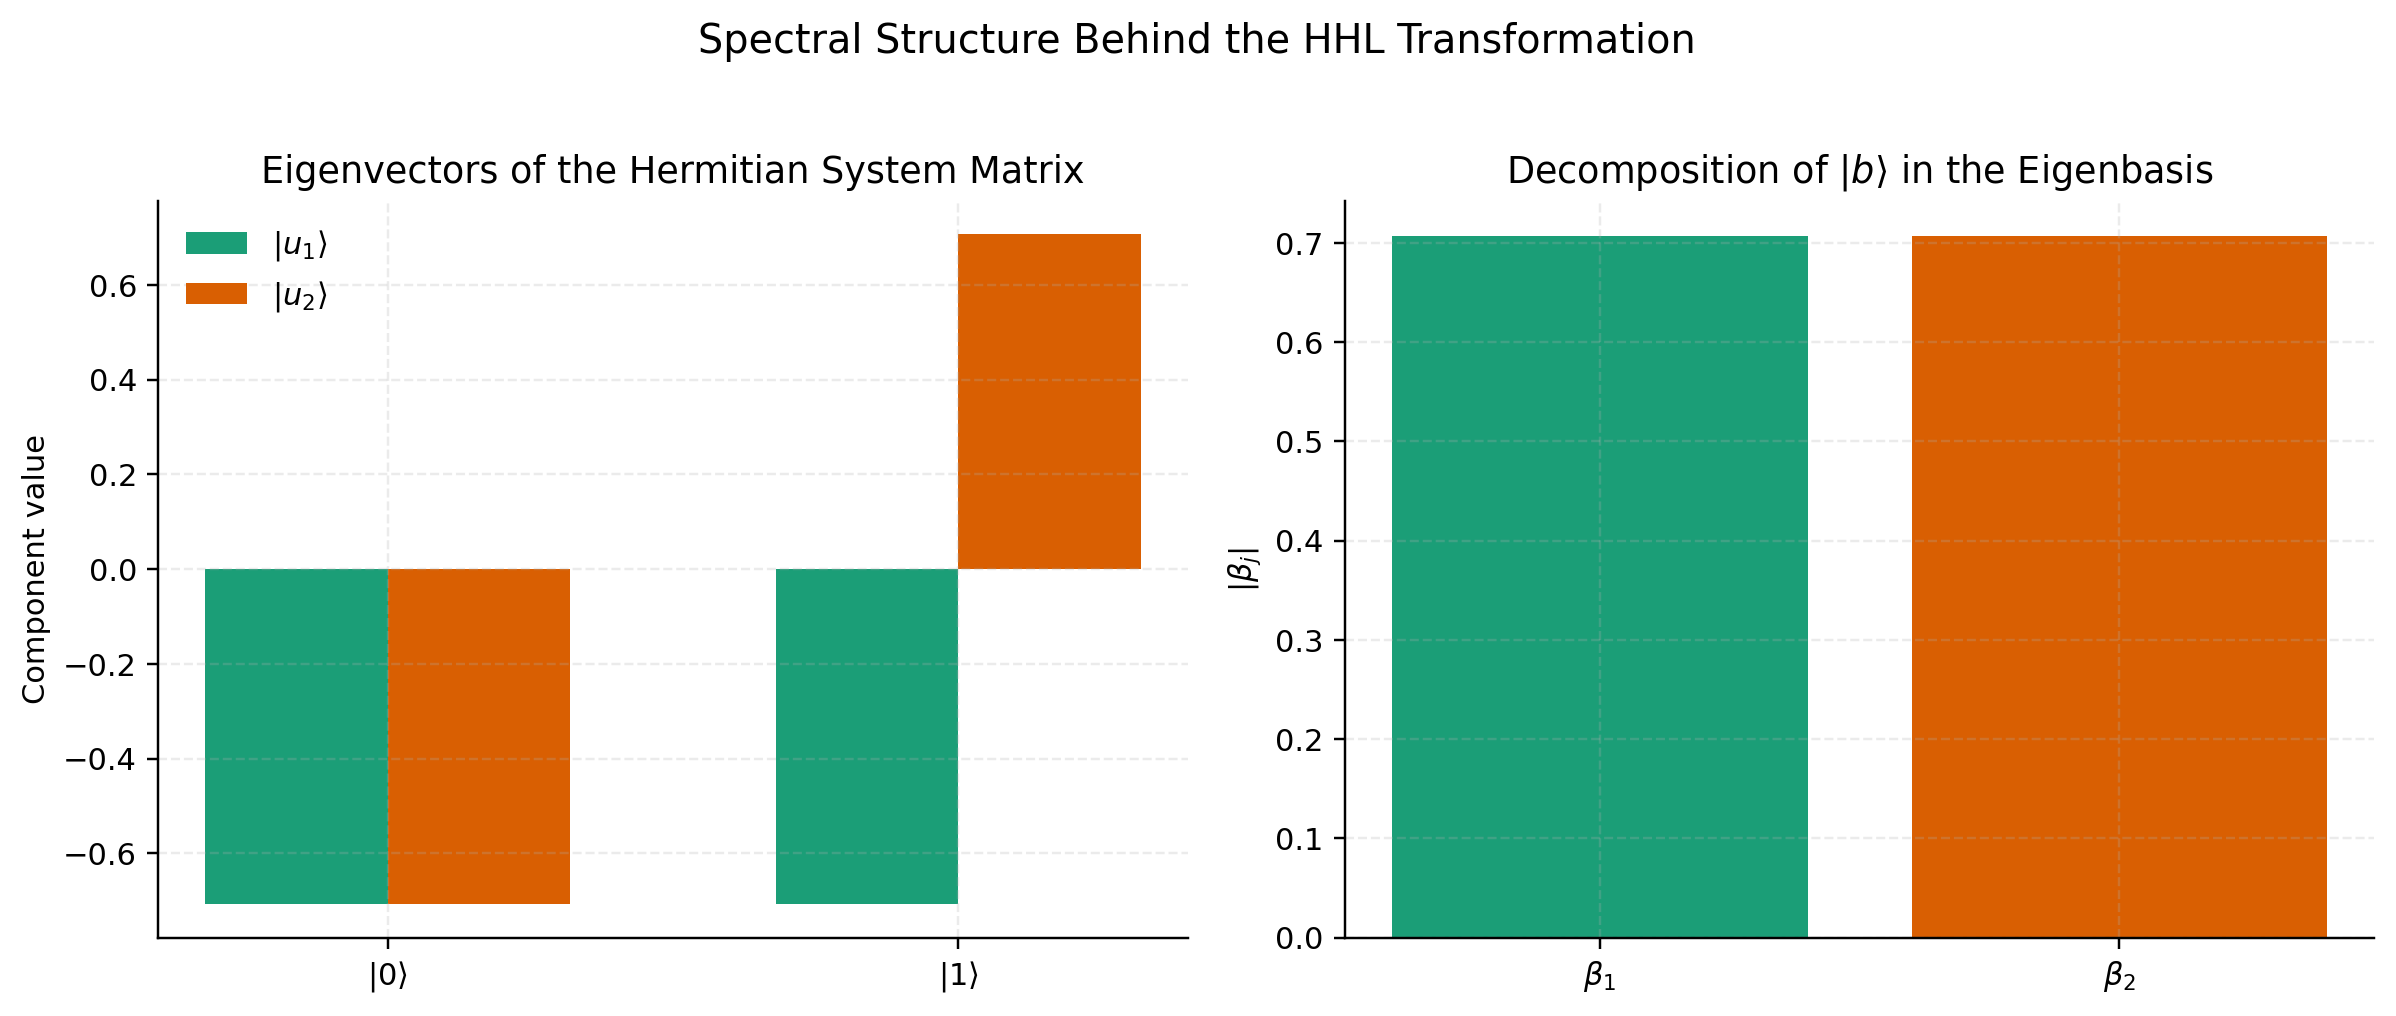
\includegraphics[width=0.92\textwidth]{figures/spectral_decomposition.png}
    \caption{Spectral decomposition of the system matrix and coefficients of the input state in the eigenbasis.}
\end{figure}

\section{Hamiltonian Simulation and Exact Two-Bit Phase Encoding}

HHL uses the unitary
\[
U = e^{iAt}.
\]
In this repository we choose
\[
t = \frac{3\pi}{4}.
\]
This makes the phase fractions
\[
\phi_j = \frac{\lambda_j t}{2\pi}
\]
exactly representable on two phase qubits:
\[
\phi_1 = \frac{1}{4},
\qquad
\phi_2 = \frac{1}{2}.
\]
Therefore quantum phase estimation maps
\[
\sum_j \beta_j |u_j\rangle |00\rangle
\longmapsto
\sum_j \beta_j |u_j\rangle |\tilde{\lambda}_j\rangle,
\]
with no discretization error for this specific choice of problem and evolution time. In the implementation, the clock states correspond to the two binary fractions associated with these exact phases.

\begin{figure}[h]
    \centering
    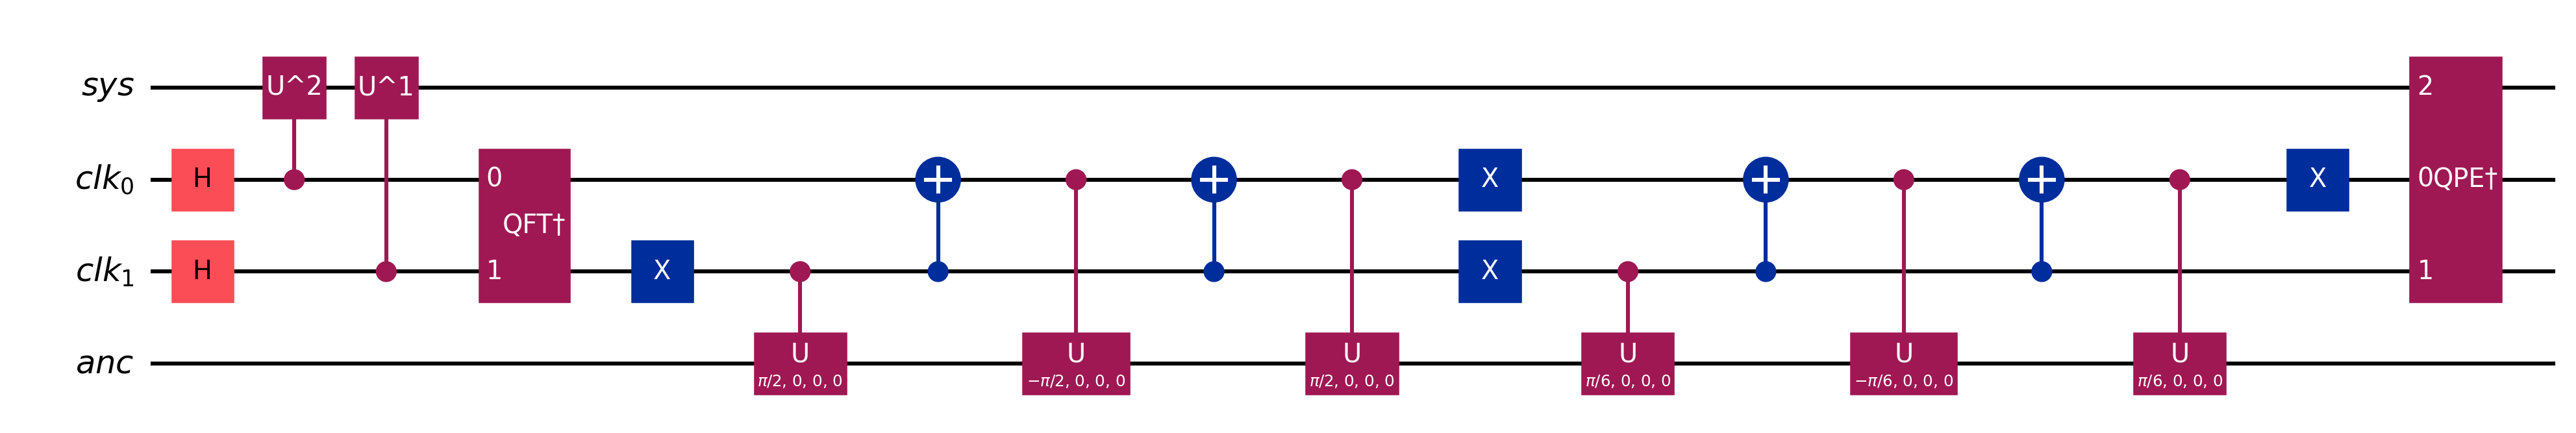
\includegraphics[width=0.95\textwidth]{figures/circuit_hhl.png}
    \caption{Executable HHL circuit produced by the package.}
\end{figure}

\begin{figure}[h]
    \centering
    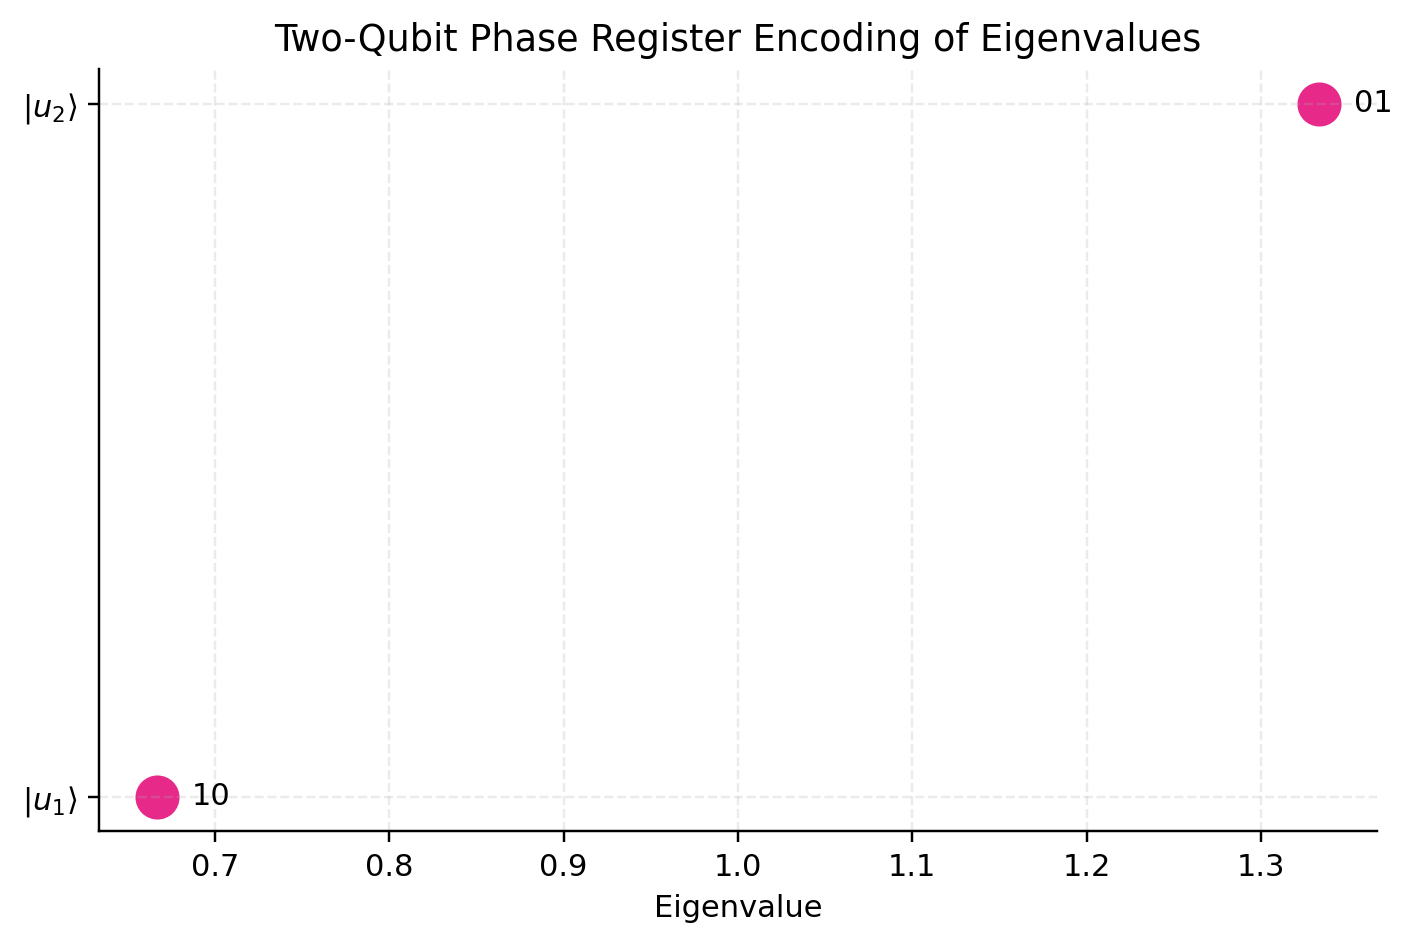
\includegraphics[width=0.70\textwidth]{figures/eigenvalue_encoding.png}
    \caption{Encoding of the two eigenvalues onto the phase register.}
\end{figure}

\section{Controlled Reciprocal Rotation}

The next step introduces an ancilla qubit and applies an eigenvalue-controlled rotation. For a scale constant $C \le \min_j \lambda_j$, the ancilla is rotated so that
\[
|0\rangle_{\mathrm{anc}}
\mapsto
\sqrt{1-\left(\frac{C}{\lambda_j}\right)^2}|0\rangle
+
\frac{C}{\lambda_j}|1\rangle.
\]
This is the stage where the reciprocal dependence on $\lambda_j$ enters the computation. In the code, the operation is implemented through basis-controlled $R_y$ rotations on the phase register.

\begin{figure}[h]
    \centering
    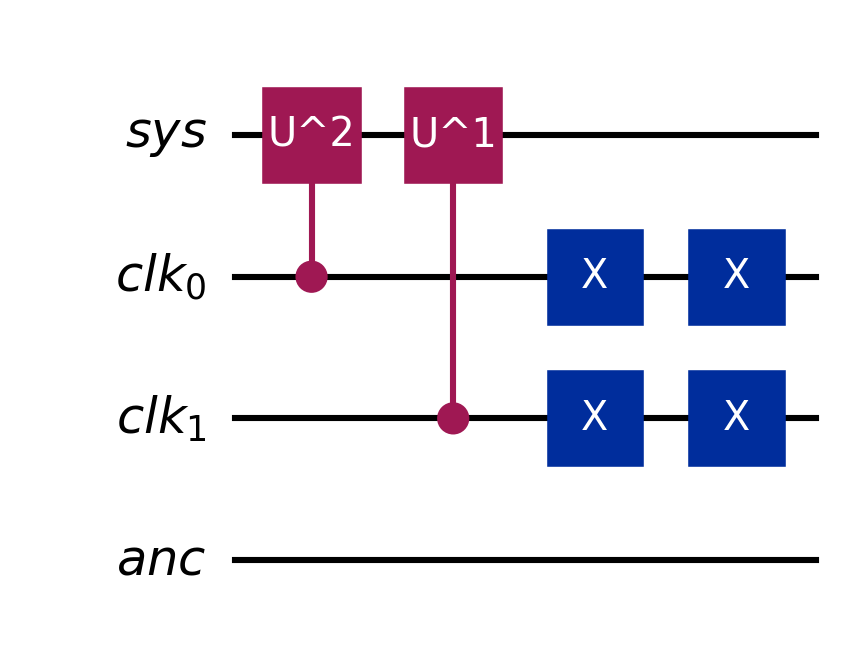
\includegraphics[width=0.76\textwidth]{figures/inversion_oracle.png}
    \caption{Basis-controlled inversion oracle implementing the reciprocal weighting.}
\end{figure}

\section{Uncomputation and Postselection}

After the reciprocal rotation, the inverse of phase estimation is applied. This erases the phase register while preserving the amplitude factors introduced on the ancilla:
\[
\sum_j \beta_j |u_j\rangle |\tilde{\lambda}_j\rangle
\longmapsto
\sum_j \beta_j |u_j\rangle |00\rangle.
\]
Conditioned on measuring the ancilla in the accepting state $|1\rangle$, the system register becomes
\[
\sum_j \beta_j \frac{C}{\lambda_j}|u_j\rangle
\propto
A^{-1}|b\rangle.
\]
The implementation makes this branch explicit by extracting only the amplitudes for which the ancilla equals $1$ and the clock register has been uncomputed back to $|00\rangle$.

\section{Recovered State and Numerical Agreement}

The raw postselected amplitudes obtained from the statevector are proportional to the classical solution:
\[
\begin{bmatrix}
3/4 \\
1/4
\end{bmatrix}
\propto
\begin{bmatrix}
9/8 \\
3/8
\end{bmatrix}.
\]
After normalization, the recovered HHL state matches the normalized classical solution,
\[
\frac{x}{\|x\|} =
\begin{bmatrix}
0.948683 \\
0.316228
\end{bmatrix},
\qquad
|x_{\mathrm{HHL}}\rangle =
\begin{bmatrix}
0.948683 \\
0.316228
\end{bmatrix}.
\]

\begin{table}[h]
    \centering
    \begin{tabular}{>{\raggedright\arraybackslash}p{0.52\textwidth}r}
        \toprule
        Quantity & Value \\
        \midrule
        Postselection success probability & 0.625000 \\
        State fidelity with normalized classical solution & 1.000000 \\
        Relative $L^2$ error & $8.29 \times 10^{-16}$ \\
        \bottomrule
    \end{tabular}
    \caption{Numerical agreement between the HHL output state and the normalized classical solution.}
\end{table}

\begin{figure}[h]
    \centering
    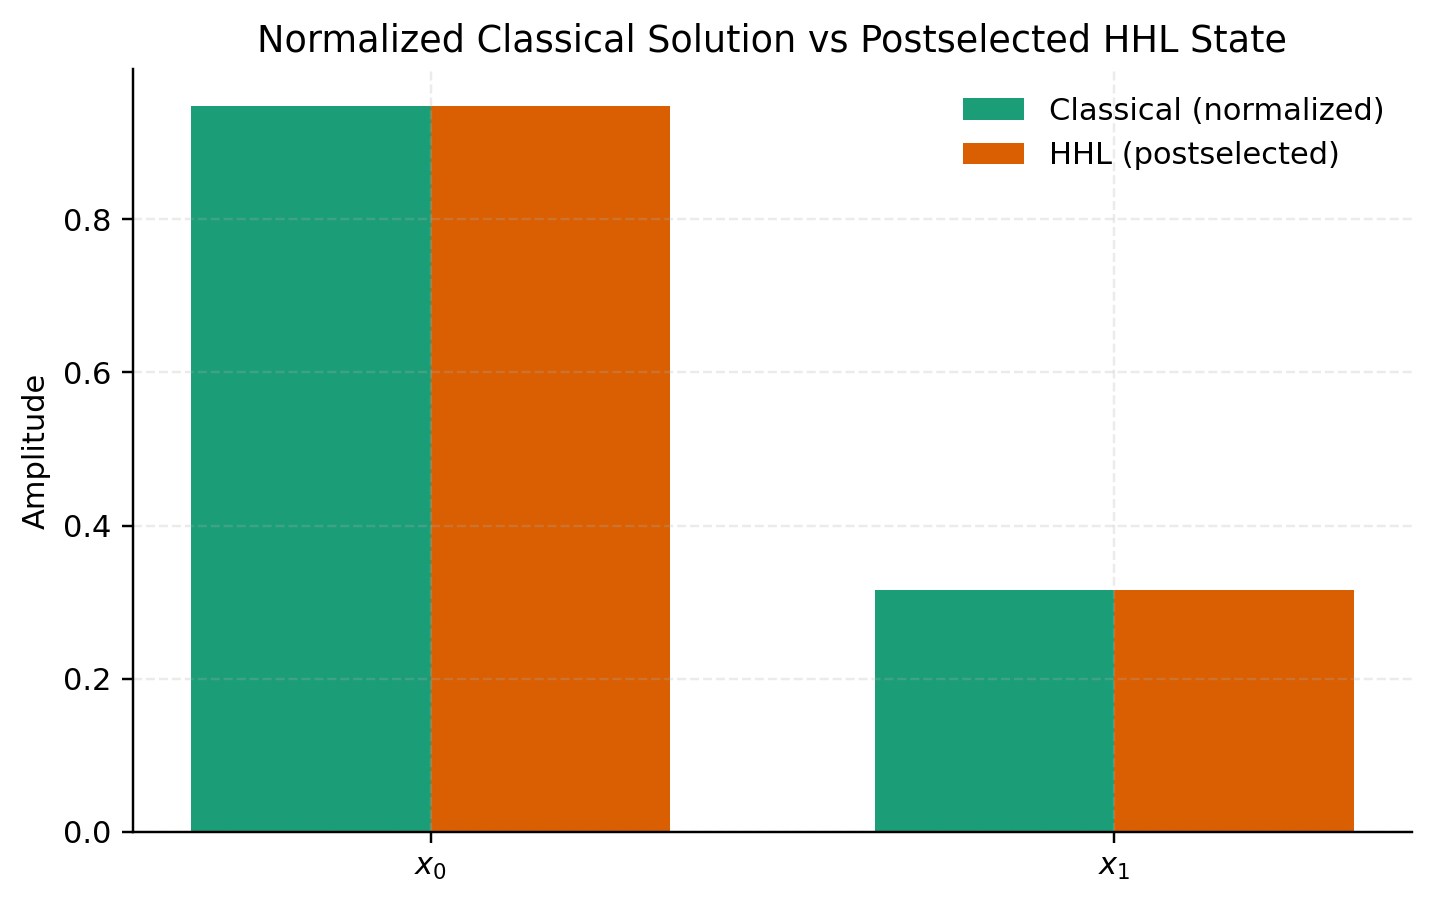
\includegraphics[width=0.76\textwidth]{figures/solution_comparison.png}
    \caption{Comparison between the normalized classical solution and the postselected HHL state.}
\end{figure}

\begin{figure}[h]
    \centering
    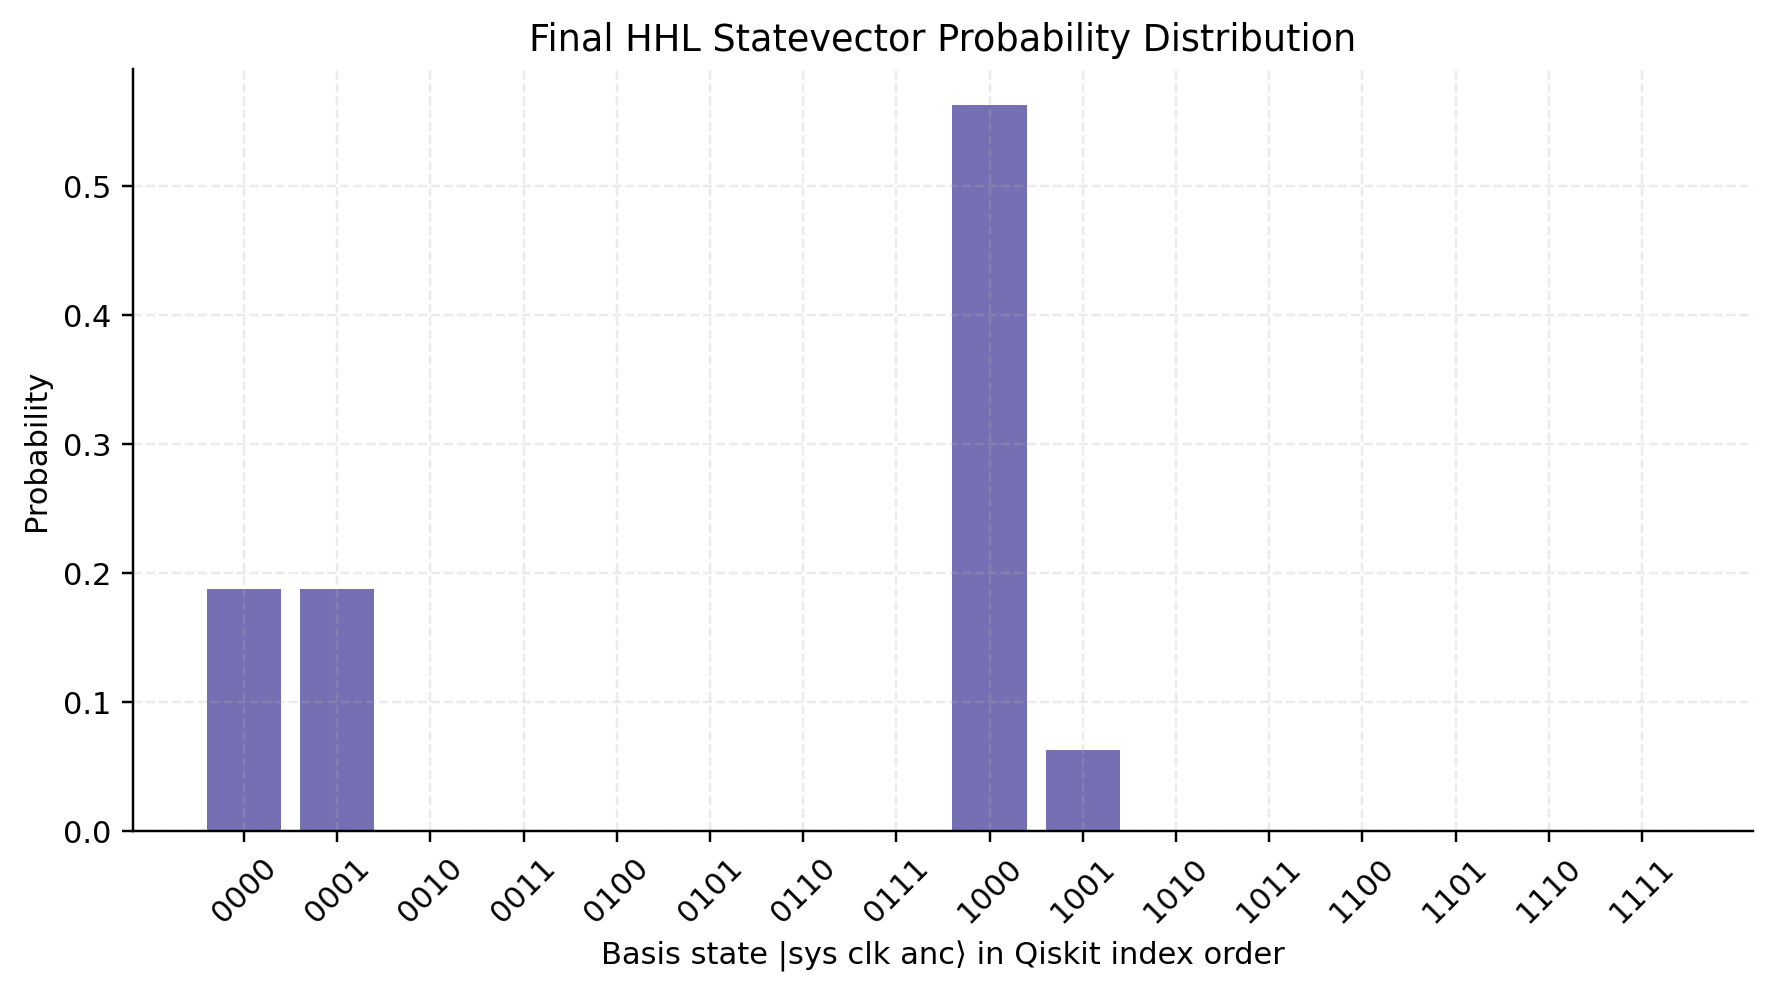
\includegraphics[width=0.76\textwidth]{figures/statevector_distribution.png}
    \caption{Probability distribution of the final four-qubit HHL statevector.}
\end{figure}

\begin{figure}[h]
    \centering
    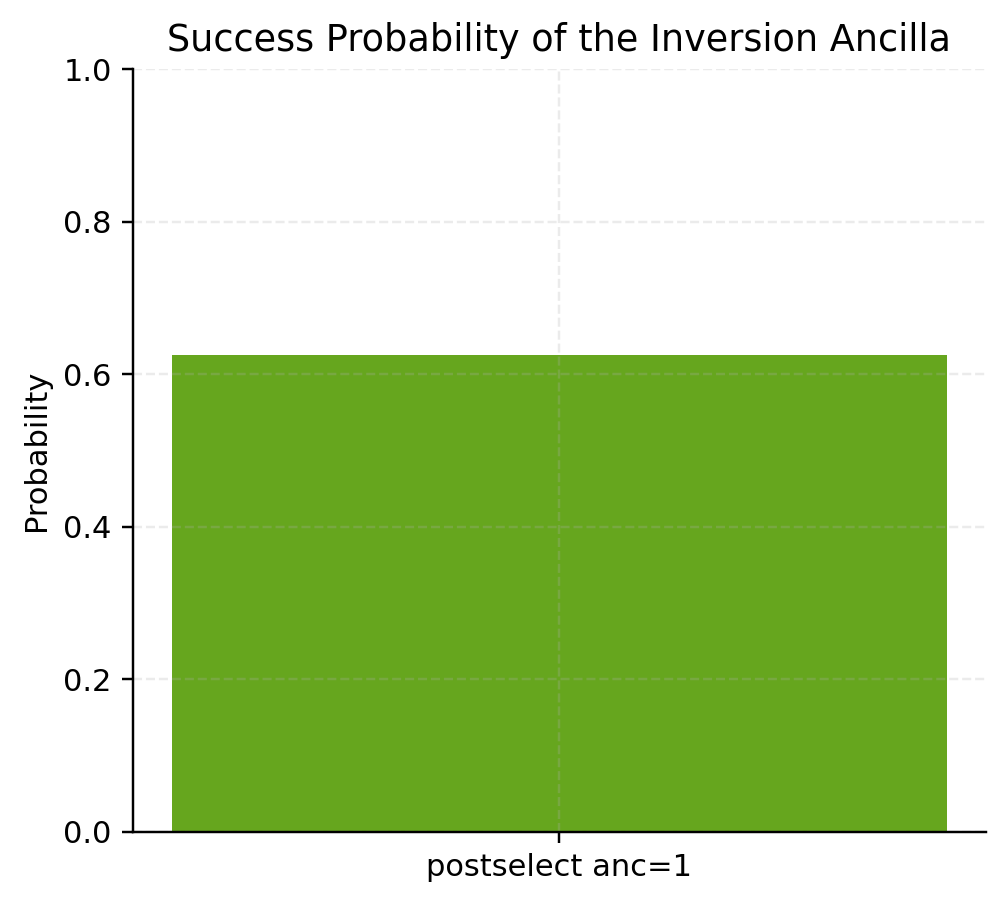
\includegraphics[width=0.54\textwidth]{figures/success_probability.png}
    \caption{Probability of observing the inversion ancilla in the accepting state.}
\end{figure}

\section{Finite-Precision Discussion}

The repository also includes a small precision study based on eigenphase discretization. For the canonical example, the conclusion is pedagogically sharp:
\begin{itemize}
    \item one phase qubit is insufficient, because the smaller phase aliases to zero and the reciprocal rotation becomes ill-defined;
    \item two phase qubits are already exact;
    \item adding more phase qubits does not improve the recovered state because the binary fractions are already represented exactly.
\end{itemize}

\begin{figure}[h]
    \centering
    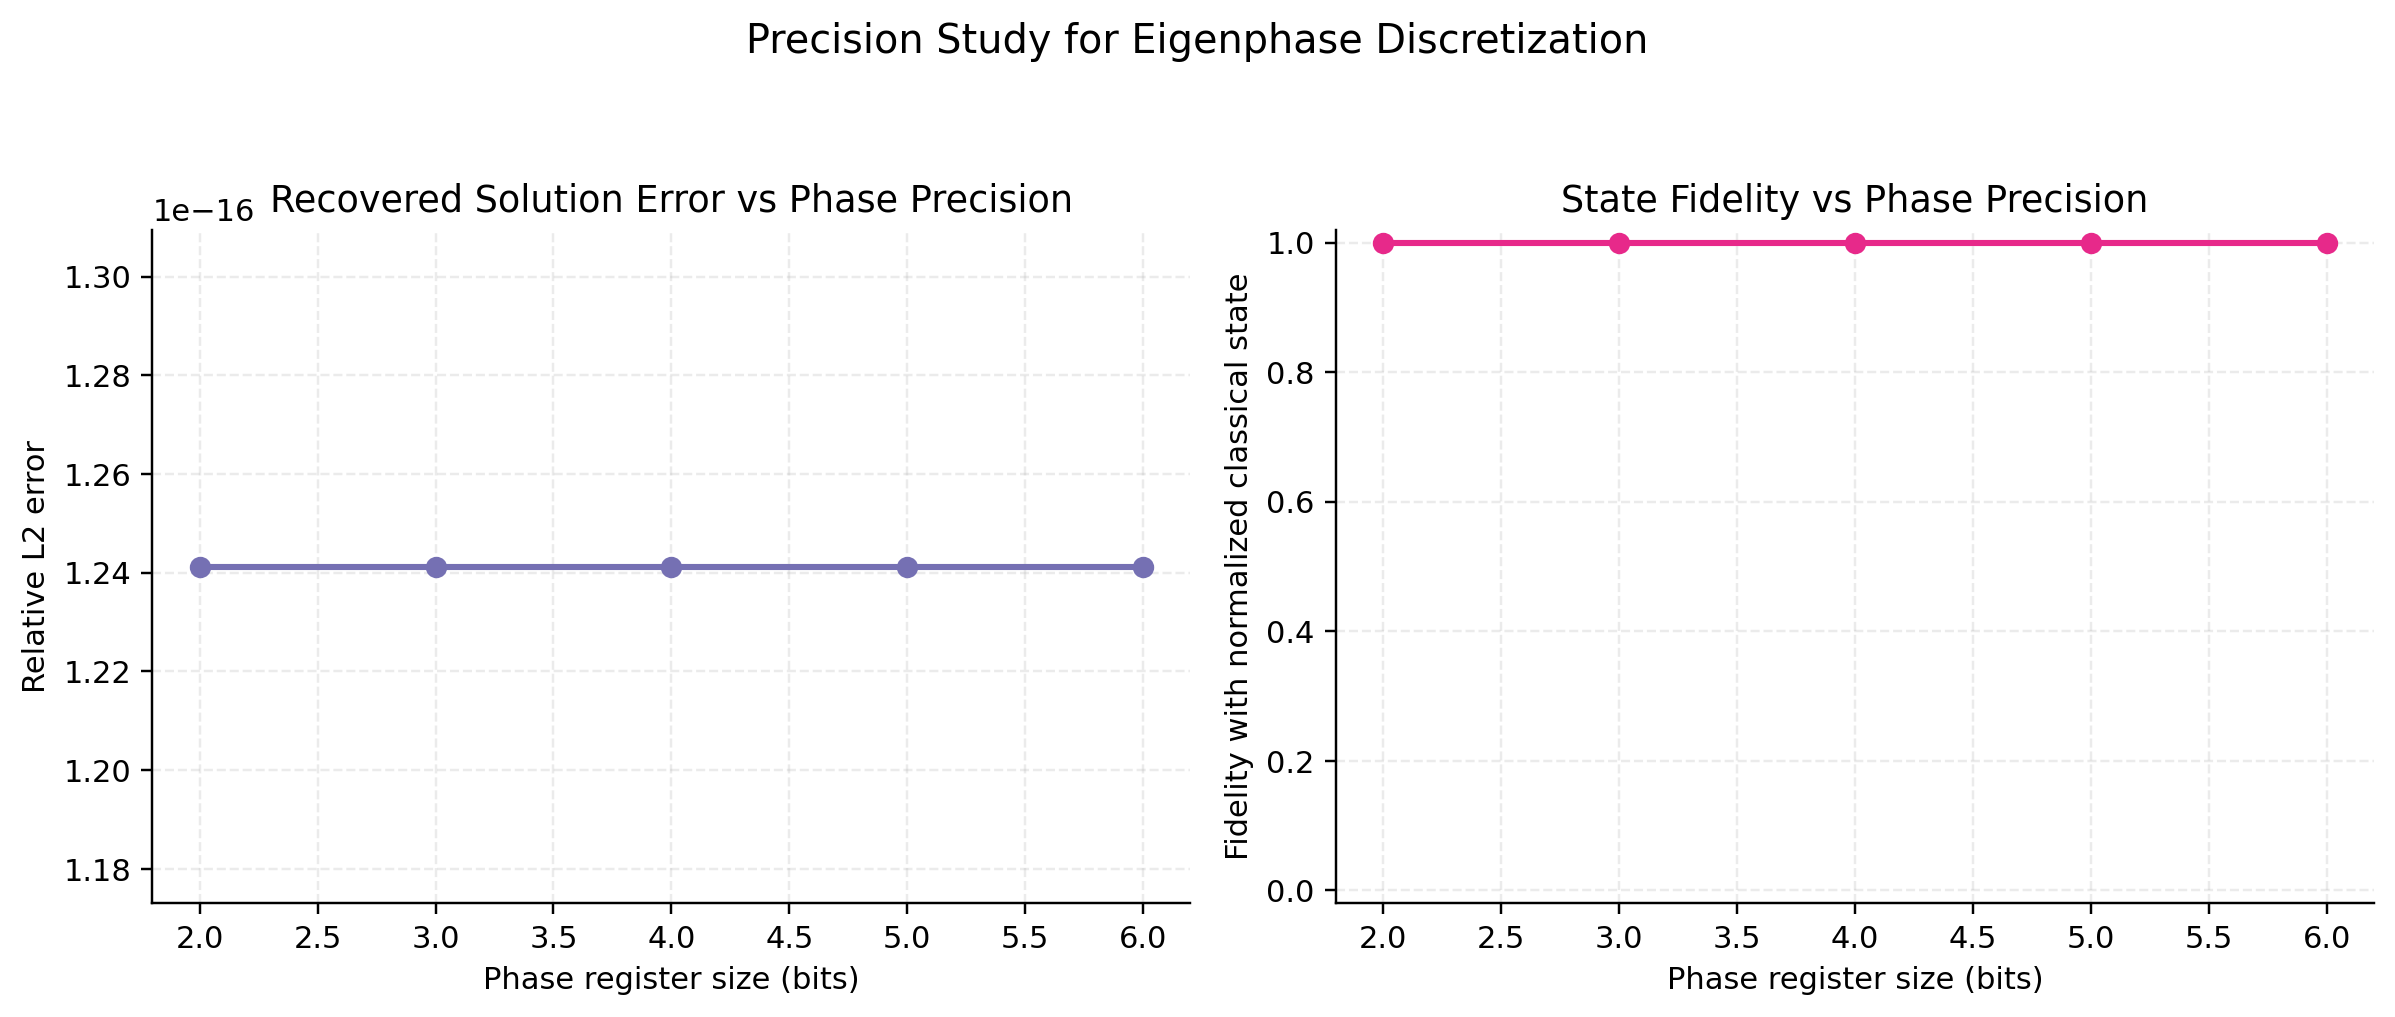
\includegraphics[width=0.92\textwidth]{figures/precision_sweep.png}
    \caption{Relative error and state fidelity as functions of phase-register size.}
\end{figure}

\section{Interpretation and Scope}

This project is intentionally modest in size but high in transparency. It does not attempt sparse-Hamiltonian scaling, block-encoding, or fault-tolerant resource estimation. Instead, it provides a bridge between the symbolic derivation of HHL and an inspectable Qiskit realization whose outputs can be checked numerically, visualized, and tested automatically.

\end{document}
